\documentclass[twoside,11pt]{article}

\usepackage{aa228-jmlr2e}
\usepackage{amsmath}
\usepackage{graphicx}
\usepackage{lipsum}
\usepackage{listings}
\usepackage{url}
\usepackage{cleveref}
\usepackage{subcaption}

\usepackage{enumitem}
\usepackage{breakurl}
\usepackage{hyperref}

\setlist[itemize]{noitemsep}  % or \setlist[itemize]{itemsep=0pt, topsep=0pt}

\begin{document}

\title{Lagrange points: a quick analysis}
\name{Stuart Johnson}
\maketitle

\section{Introduction}
The analysis below is the start of a project whose goal is the modeling of spacecraft control near Lagrange points in Simulink and Modelica. All mathematical and theoretical mistakes are to be blamed on the author! This analysis was inspired by Scott Manley's video on YouTube (\cite{Manley}). Also see \cite{Baez} for some nice background.

% move this to references
%Scott Manley. "What Makes Lagrange Points Special Locations In Space" YouTube, Oct. 15 2021, https://www.youtube.com/watch?v=7PHvDj4TDfM&t=681s.

\section{Forces in a 2-body system in uniform circular motion about the center of mass}

A two-body system of masses $m_0$ and $m_1$ in uniform circular motion in the $x-y$ plane about their center of mass at $(0,0)$ can be described in a co-rotating coordinate system such that


\begin{align}
\vec{r}_0 &= (-x_0,0), x_0 > 0 \nonumber \\ 
\vec{r}_1 &= (x_1,0), x_1 > 0 \nonumber
\end{align}


define the positions of the corresponding masses. In this co-rotating coordinate system, each stationary (in uniform circular motion) mass is subject to two forces: the gravitational force $\vec{f}_g$ due to all the other masses, and the fictitious centrifugal force $\vec{f}_c$ due to the fact that the co-rotating coordinate system is not an inertial reference frame. In particular, our two masses $m_0$ and $m_1$ must each experience $0$ total force:

\begin{equation}
0 = \vec{f}_c + \vec{f}_g  \label{eq:totalforce}
\end{equation}

Note that real two-body systems do not exist in isolation, do not quite orbit in a single plane, and are not populated by bodies following circular orbits! So we are simplifying the system for a simple mathematical treatment.

Since both objects are rotating at constant angular velocity $\omega$, equation \eqref{eq:totalforce} yields the following for masses $m_0$ and $m_1$, respectively:
\begin{align}
m_0 \omega^2 x_0 &= \frac{G m_0 m_1}{\left( x_0 + x_1 \right)^2} \label{eq:mass0} \\
m_1 \omega^2 x_1 &= \frac{G m_0 m_1}{\left( x_0 + x_1 \right)^2} \label{eq:mass1}
\end{align}

Dividing equation \eqref{eq:mass0} by equation \eqref{eq:mass1} results in the relation between masses $m_0$ and $m_1$ and their fixed positions in co-rotating space:
\begin{equation}
\frac{x_0}{x_1} = \frac{m_1}{m_0} \label{eq:positions}
\end{equation}

We are free to choose any separation distance $ d = x_0 + x_1 $. If our masses are point masses (see below), $ \omega $ is entirely defined by our mass configuration via equations \eqref{eq:mass0} and \eqref{eq:mass1}. Furthermore, we have, from equation \eqref{eq:positions}:

\begin{align}
x_0 &= \left. d \middle/ \left(1 + \frac{m_0}{m_1} \right) \right. \nonumber \\ 
x_1 &= \frac{m_0}{m_1} x_0 \nonumber
\end{align}

In particular, the case $ d = 1 $ is handy (see below).

In order to define the Lagrange points, let's consider the force on an infinitesimal mass [Scott Manley, 2021] $m$ at position $\vec{r} = r\hat{r}$. For $m$ in uniform circular motion about the center of mass of $m_0$ and $m_1$, we have the force equation:

\begin{equation}
\vec{f} = \vec{f}_c\left(m,r\right) - \vec{f}_g\left(m, m_0, \vec{r}-\vec{r}_0\right) - \vec{f}_g\left(m, m_1, \vec{r}-\vec{r}_1\right) \label{eq:mforce}
\end{equation}

Note that since this infinitesimal mass $m$ is stationary in the co-rotating frame, there are no other fictitious forces acting on it. For example, if $m$ had non-zero velocity in the co-rotating frame, it would experience a Coriolis force as well. Also, the fact that $m$ is far less than either $m_0$ or $m_1$ allows us to ignore it's negligible contribution to the spatial configuration of this system of bodies. Finally, we are considering all masses to be point masses; the formulas for $\vec{f}_g$ do not hold within the physical extent of the masses (amongst other issues!).

Writing out equation \eqref{eq:mforce} in it's full glory results in:
\begin{equation}
\vec{f} = m \omega^2 \vec{r} - G m m_0 \frac{\vec{r}-\vec{r}_0}{\left|\vec{r}-\vec{r}_0\right|^3} - G m m_1 \frac{\vec{r}-\vec{r}_1}{\left|\vec{r}-\vec{r}_1\right|^3} \label{eq:fullglory}
\end{equation}

We can use equations \eqref{eq:mass0} and \eqref{eq:mass1} to entirely recast equation \eqref{eq:fullglory} in terms of locations in co-rotating space:

\begin{equation}
\vec{f} = m \omega^2 \vec{r} - m \omega^2 x_1 \left( x_0 + x_1 \right)^2 \frac{\vec{r}-\vec{r}_0}{\left|\vec{r}-\vec{r}_0\right|^3} - m \omega^2 x_0 \left( x_0 + x_1 \right)^2 \frac{\vec{r}-\vec{r}_1}{\left|\vec{r}-\vec{r}_1\right|^3} \label{eq:fullglorysimp1}
\end{equation}

Dividing out common non-zero factors yields:

\begin{equation}
\vec{f}\left(\vec{r}\right) \propto \vec{r} - x_1 \left( x_0 + x_1 \right)^2 \frac{\vec{r}-\vec{r}_0}{\left|\vec{r}-\vec{r}_0\right|^3} - x_0 \left( x_0 + x_1 \right)^2 \frac{\vec{r}-\vec{r}_1}{\left|\vec{r}-\vec{r}_1\right|^3} \label{eq:fullglorysimp2}
\end{equation}

A convenient coordinate system for solving (and plotting!) equation \eqref{eq:fullglorysimp2} is the normalized, translated coordinate system

\begin{equation}
\vec{r}\thinspace' = \frac{\vec{r}+\left(x_0,0\right)}{x_0 + x_1} \label{eq:normcoordsys}
\end{equation}

which places $m_0$ (at $(-x_0,0)$ in the center of mass coordinate system) at the origin and $m_1$ at ${\vec{r}}_{1}\thinspace' = \left(1,0\right)$.

\section{Lagrange points in a 2-body system in uniform circular motion about the center of mass}

Solutions $\vec{r}$ of 
\begin{equation}
\vec{f}\left(\vec{r}\right) = 0 \label{eq:forcesolutions}
\end{equation}

are the Lagrange points of this 2-body system. Squinting at equation \eqref{eq:fullglorysimp2} suggests that if 
\begin{equation}
\left|\vec{r}-\vec{r}_0\right| = \left|\vec{r}-\vec{r}_1\right|
\end{equation}
many terms will cancel out. A little more experimentation reveals that, indeed, if
\begin{equation}
\left|\vec{r}-\vec{r}_0\right| = \left|\vec{r}-\vec{r}_1\right| = x_0 + x_1
\end{equation}

equation \ref{eq:forcesolutions} is satisfied. These are two Lagrange points forming an equilateral triangle in $x-y$ location with $m_0$ and $m_1$. These are, by convention, referred to as $L_4$ and $L_5$, and are invariant to the mass ratio of $m_0$ and $m_1$ - although the shape of the forces \textit{near} $L_4$ and $L_5$ is heavily influenced by the mass ratio.

A little plotting of $\log\left(\left|\vec{f}\right|\right)$ (see figures below) reveals three additional Lagrange points along the $x$-axis of the co-rotating coordinate system. These three solutions lie to either side of $m_0$ and $m_1$ and another between the two masses. The solution for these Lagrange points are the roots of a fifth-order equation in $x$. It is a straightforward matter to use a numerical solver to obtain these three Lagrange points. Especially convenient is a solver (such as MATLAB's fzero()) which accepts the root brackets, specifically:

\begin{equation}
f_x(x) = 0 \quad \text{s.t.} \begin{cases}
     -x_0 - n (x_0+x_1) < x < -x_0 - \epsilon &\text{for $L_3$}\\
     -x_0 + \epsilon < x < x_1 - \epsilon &\text{for $L_1$}\\
     x_1 + \epsilon < x < x_1 + n (x_0+x_1) &\text{for $L_2$}
  \end{cases} \nonumber
\end{equation}

since $\vec{f}$ only has an $x$-component when evaluated at points on the $x$-axis. Note that the outer root limits have been set using $n=2$, or $\pm 2 (x_0+x_1)$ in the MATLAB code. It should be sufficient to use $\pm (x_0+x_1)$, or $n=1$.

The Lagrange point table below shows the result of root finding for Lagrange points $L_1$ - $L_3$ and the invariant $L_4$ and $L_5$ points for a range of mass ratios. The last two two-body systems are fictitious, and meant to show what happens at mass ratios near unity. The $x$ and $y$ coordinates in the table are in the normalized, shifted coordinate system such that $m_0$ is located at $\left(0,0\right)$ and $m_1$ is located at $\left(1,0\right)$.

These 4 systems (with a zoom on the Sun-Earth system near the earth) are shown in the following plots of force magnitude and table of locations of force zero solutions (\ref*{tab:lagpoints}).

\begin{minipage}{\textwidth}
	\begin{center}
		\begin{tabular}{llllllll}
system & m0/m1 & coord & L1 & L2 & L3 & L4 & L5 \\ 
\hline 
Earth-Moon & 81.3 & x & 0.84907 & 1.1678 & -0.99291 & 0.5 & 0.5 \\ 
Earth-Moon & 81.3 & y & 0 & 0 & 0 & 0.86603 & -0.86603 \\ 
Sun-Earth & 330000 & x & 0.99 & 1.0101 & -1 & 0.5 & 0.5 \\ 
Sun-Earth & 330000 & y & 0 & 0 & 0 & 0.86603 & -0.86603 \\ 
m0-m1 & 5 & x & 0.65856 & 1.4381 & -0.9025 & 0.5 & 0.5 \\ 
m0-m1 & 5 & y & 0 & 0 & 0 & 0.86603 & -0.86603 \\ 
m0-m1 & 1 & x & 0.5 & 1.6984 & -0.69841 & 0.5 & 0.5 \\ 
m0-m1 & 1 & y & 0 & 0 & 0 & 0.86603 & -0.86603 \\ 
\hline 
\end{tabular}
		\captionof{table}{Lagrange points for 4 systems of interest. Coordinates are in the normalized coordinate system (equation \eqref{eq:normcoordsys}).}
		\label{tab:lagpoints}
	\end{center}
\end{minipage}

\begin{minipage}{\textwidth}
	\begin{center}
		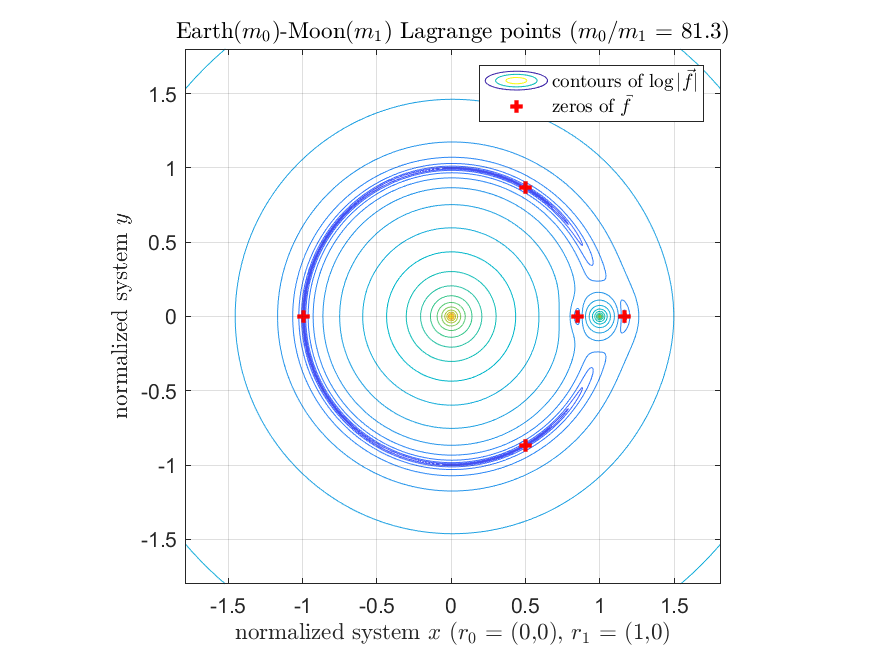
\includegraphics[width=0.8\linewidth]{../Earth-Moon.png}
		\captionof{figure}{Force magnitude for the Earth-Moon system.}
		\label{fig:earthmoon}
	\end{center}
\end{minipage}

\begin{minipage}{\textwidth}
	\begin{center}
		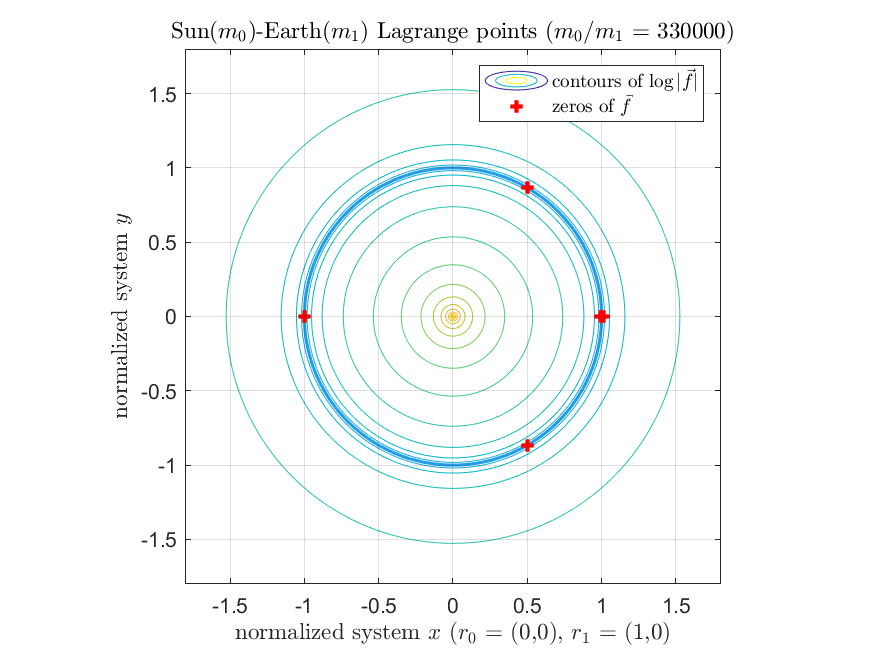
\includegraphics[width=0.8\linewidth]{../Sun-Earth.png}
		\captionof{figure}{Force magnitude for the Sun-Earth system.}
		\label{fig:sunearth}
	\end{center}
\end{minipage}

\begin{minipage}{\textwidth}
	\begin{center}
		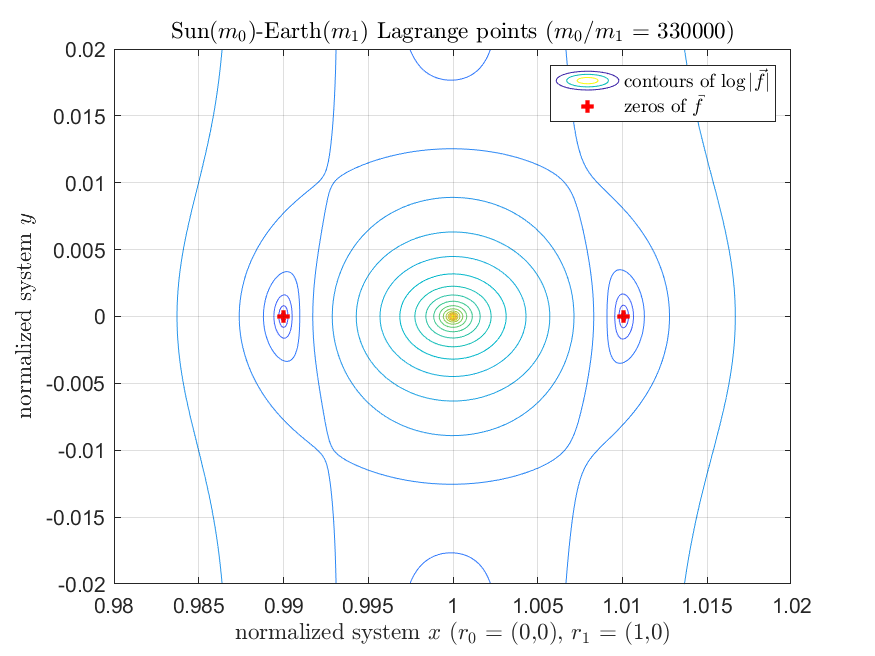
\includegraphics[width=0.8\linewidth]{../Sun-Earth_zoom.png}
		\captionof{figure}{Force magnitude for the Sun-Earth system (zoomed on Earth).}
		\label{fig:sunearth}
	\end{center}
\end{minipage}

\begin{minipage}{\textwidth}
	\begin{center}
		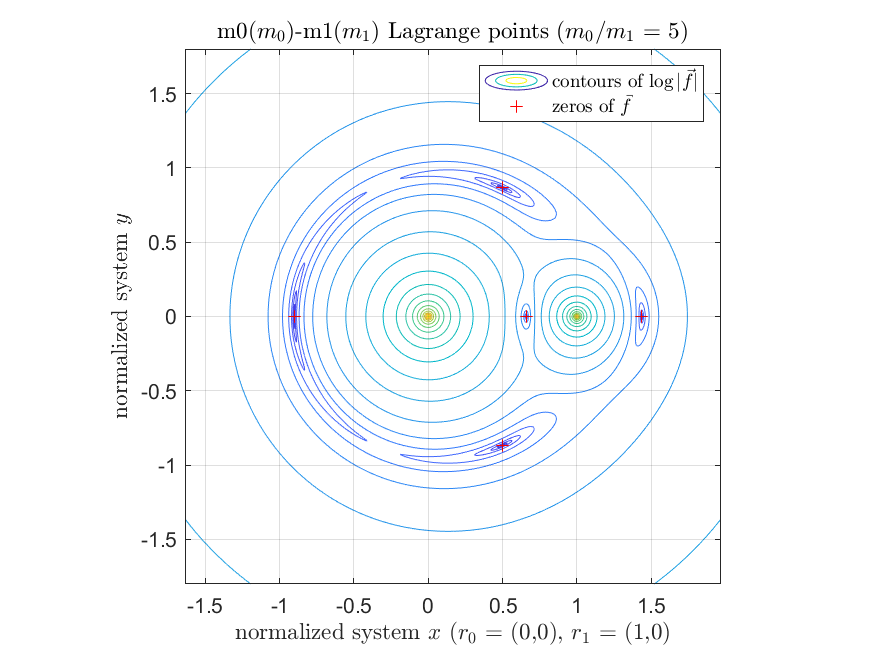
\includegraphics[width=0.8\linewidth]{../m0-m1_mr5.png}
		\captionof{figure}{Force magnitude for a fictitious system with mass ratio of 5.}
		\label{fig:sunearth}
	\end{center}
\end{minipage}

\begin{minipage}{\textwidth}
	\begin{center}
		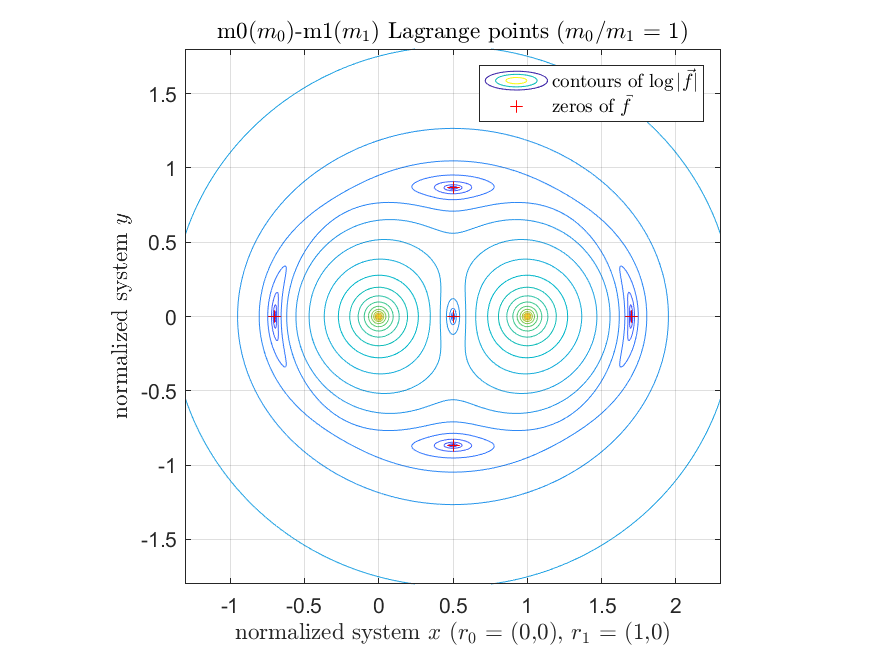
\includegraphics[width=0.8\linewidth]{../m0-m1_mr1.png}
		\captionof{figure}{Force magnitude for a fictitious system with mass ratio of 1.}
		\label{fig:sunearth}
	\end{center}
\end{minipage}


% References
\bibliography{references}

\end{document}

